\documentclass[a4paper]{article}

%% Language and font encodings
\usepackage[english]{babel}
\usepackage[utf8x]{inputenc}
% \usepackage[T1]{fontenc}
\usepackage{float}
\usepackage{url}

\usepackage{helvet}
\renewcommand{\familydefault}{\sfdefault}

%% Sets page size and margins
\usepackage[a4paper,top=3cm,bottom=2cm,left=3cm,right=3cm,marginparwidth=1.75cm]{geometry}

%% Useful packages
\usepackage{amsmath}
\usepackage{graphicx}
\usepackage[colorinlistoftodos]{todonotes}
\usepackage[colorlinks=true, allcolors=blue]{hyperref}

\usepackage{listings}
\lstset{basicstyle=\ttfamily,
  showstringspaces=false,
  commentstyle=\color{blue},
  keywordstyle=\color{black}
}

\title{Exercise 4: Training End-to-end driving networks}
\author{Michael Floßmann, Kshitij Sirohi, Hendrik Vloet}
\pagestyle{empty}
\begin{document}
\maketitle

\section{Introduction}
\subsection{Goals}
The main objective of this assignment was to get to know the rAIScar hardware
and apply the things learned in the previous exercises to port the ML algorithm
to the platform. This included:
\begin{itemize}
\item Finish unfinished tasks from the previous exercise sheet
\item Get familiar with the rAIScar hardware to collect the training data
  (collecting and converting data for the training infrastructure)
\end{itemize}

\section{Training hyperparameters}

The hyperparameters for the training are listed in table \ref{tab:hyperpars}.

\begin{table}[H]
  \centering
  \caption{Training hyperparameters}
  \label{tab:hyperpars}
  \begin{tabular}{lc}
    $\lambda_{\mathrm{steer}}$ & 0.75 \\
    $\lambda_{\mathrm{acc}}$ & 0.25 \\
  \end{tabular}
\end{table}

\section{Leftover tasks from Exercise 3}
\subsection{Previous Issues and Observations}
There were several issues to overcome which weren't completely solved in time.
One big issue was that the meaning of the braking information was quite cryptic
and after asking the original paper authors of \cite{imitation}, it turned out
that the braking and acceleration data was supposed to be fused into one
variable. After this was done, the networks trained properly, as can be seen in
the loss plots (figures \ref{fig:augmented_command_loss}, \ref{fig:unaugmented_command_loss},
\ref{fig:augmented_branched_loss}, \ref{fig:unaugmented_branched_loss}).

The errors for the test set are shown in tables \ref{tab:error_command_aug} and \ref{tab:error_branched}.% TODO
\begin{table}[H]
  \centering
  \caption{Error values for the simulated command input net}
  \label{tab:error_command_aug}
  \begin{tabular}{lccc|ccc}
    &\multicolumn{3}{c|}{Augmented} & \multicolumn{3}{c}{Unaugmented} \\
    & MSE & Median error & Truth squared & MSE & Median error & Truth squared\\ \hline
    Steer & 0.02319 & 0.00239 & 0.03625 & 0.02947 & -0.00194 & 0.03625 \\
    Gas & 0.14106 & 0.04894 & 0.54770 & 0.17373 & 0.05971 & 0.54770
  \end{tabular}
\end{table}
\begin{table}[H]
  \centering
  \caption{Error values for the simulated branched net}
  \label{tab:error_branched}
  \begin{tabular}{lccc|ccc}
    &\multicolumn{3}{c|}{Augmented} & \multicolumn{3}{c}{Unaugmented} \\
    & MSE & Median error & Truth sqared & MSE & Median error & Truth squared\\ \hline
    Steer & 0.01987 & -0.16174 & 0.03625 & 0.01807 & -0.14034 & 0.0362544 \\
    Gas & 0.1402119 & -0.29526 & 0.54770 & 0.13247 & -0.79884 & 0.54770
  \end{tabular}
\end{table}
\begin{figure}[!htbp]
  \centering
  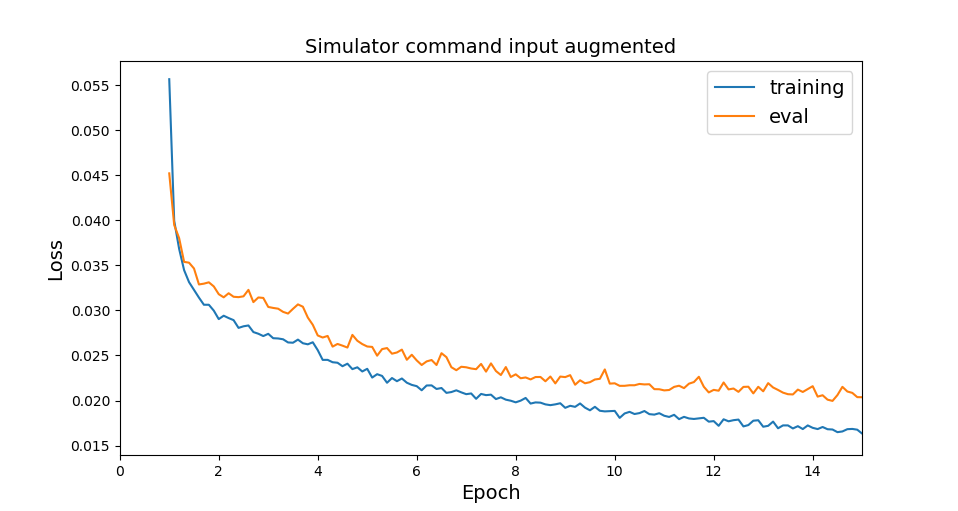
\includegraphics[width=0.95\textwidth]{figures/sim_command_input_aug_lossplot}
  \caption{Simulation command input lossplot}
  \label{fig:augmented_command_loss}
\end{figure}
\begin{figure}[!htbp]
  \centering
  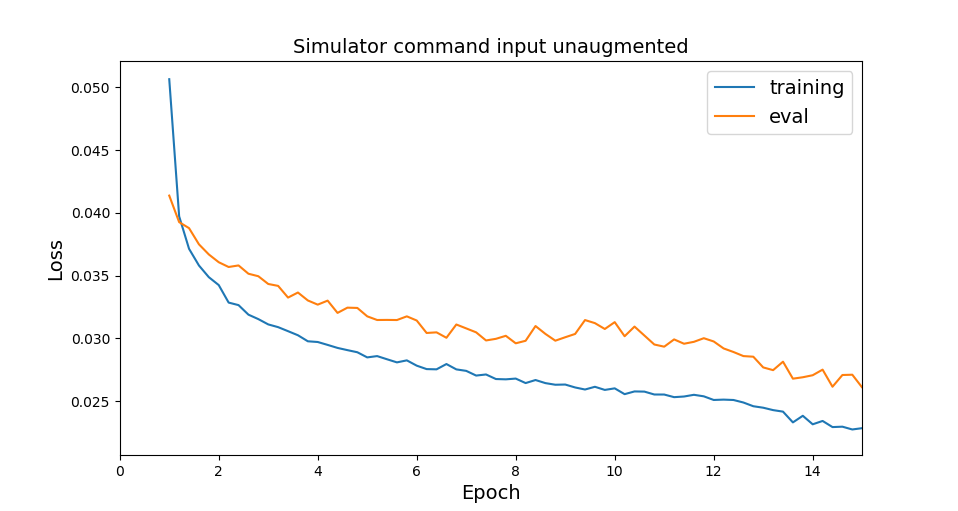
\includegraphics[width=0.95\textwidth]{figures/sim_command_input_nonaug_lossplot}
  \caption{Simulation command input, unaugmented lossplot}
  \label{fig:unaugmented_command_loss}
\end{figure}
\begin{figure}[!htbp]
  \centering
  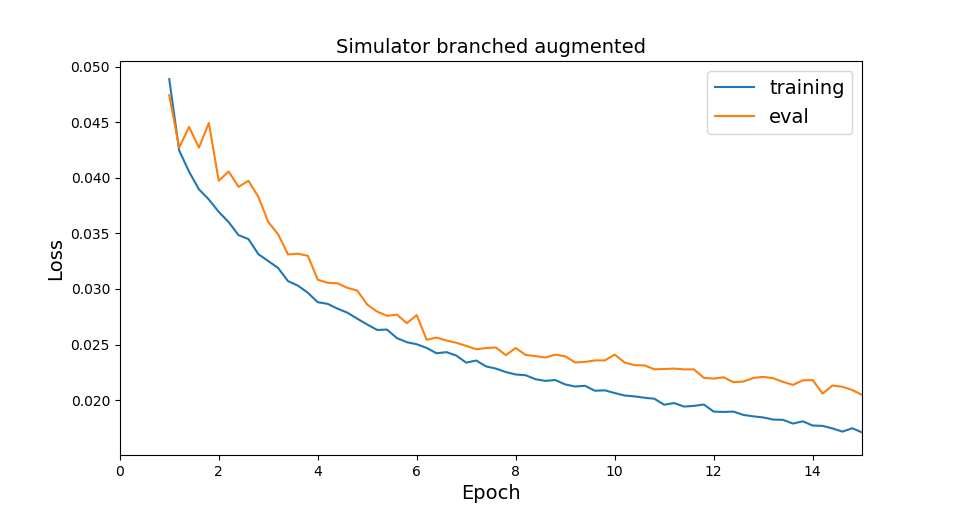
\includegraphics[width=0.95\textwidth]{figures/sim_branched_aug_lossplot}
  \caption{Simulation branched lossplot}
  \label{fig:augmented_branched_loss}
\end{figure}
\begin{figure}[!htbp]
  \centering
  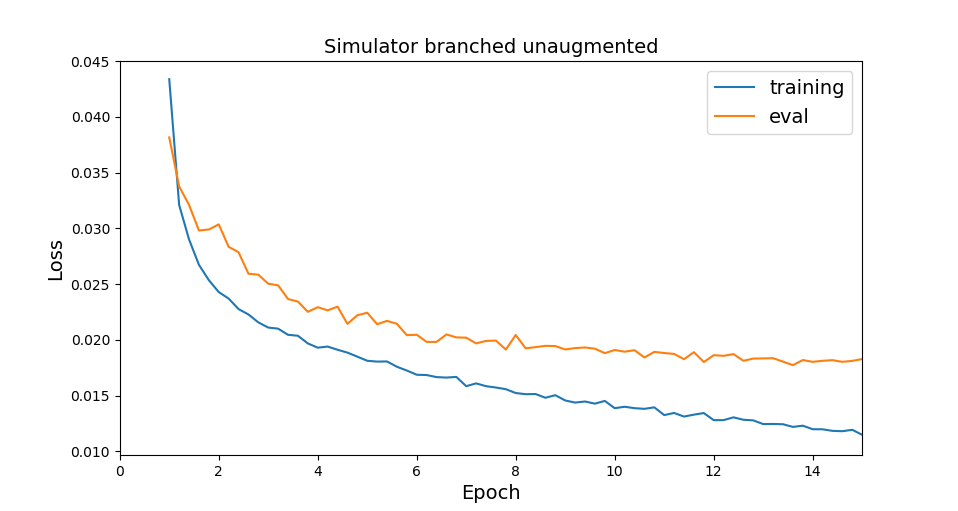
\includegraphics[width=0.95\textwidth]{figures/sim_branched_nonaug_lossplot}
  \caption{Simulation branched, unaugmented lossplot}
  \label{fig:unaugmented_branched_loss}
\end{figure}

\subsection{Interpretation}
In general, the branched network shows a lower training, validation and testing
error than the command-input network. The end result for the evaluation error in
the command input aren't too significant, which would suggest that the
augmentation-hyperparameters could be optimized still.

For the branched input, a visible improvement can be seen with augmentations, as
the evaluation and training error drift apart at the end of the 14th epoch,
suggesting overfitting.
\newpage{}
\section{Klinikum run}
For our rAIScar dataset, we went to the Uniklinikum Freiburg, because the roads
there are narrow enough and there aren't too many bystanders which would disturb
the network.

For training, we wrote a python script, converting the rosbag files from the run
into h5 datasets in the form of the simulation.

\subsection{Observations}
The errors for the test from the klinikum set are shown in tables
\ref{tab:error_command_aug_klinikum} and \ref{tab:error_branched_aug_klinikum}.

\begin{table}[H]
	\centering
	\caption{Error values for the raiscar command input klinikum net}
	\label{tab:error_command_aug_klinikum}
	\begin{tabular}{lccc|ccc}
		&\multicolumn{3}{c|}{Augmented} & \multicolumn{3}{c}{Unaugmented} \\
		& MSE & Median error & Truth squared & MSE & Median error & Truth squared\\ \hline
		Steer & 0.23373 & -0.45574 & 0.02211 & 0.04986 & -0.03150 & 0.02212 \\
		Gas & 0.04139 & -0.04197 & 0.03715 & 0.03595 & -0.01406 & 0.03715
	\end{tabular}
\end{table}
\begin{table}[H]
	\centering
	\caption{Error values for the raiscar branched klinikum net}
	\label{tab:error_branched_aug_klinikum}
	\begin{tabular}{lccc|ccc}
		&\multicolumn{3}{c|}{Augmented} & \multicolumn{3}{c}{Unaugmented} \\
		& MSE & Median error & Truth squared & MSE & Median error & Truth squared\\ \hline
		Steer & $0.04905$ & $-0.026690$ & $0.02211$ & $0.05199$ & $-0.03564$ & $0.02211$ \\
		Gas & $0.03652$ & $0.00254$ & $0.03715$ & $0.03229$ & $0.01118$ & $0.03715$
	\end{tabular}
\end{table}

\begin{figure}[!htbp]
  \centering
  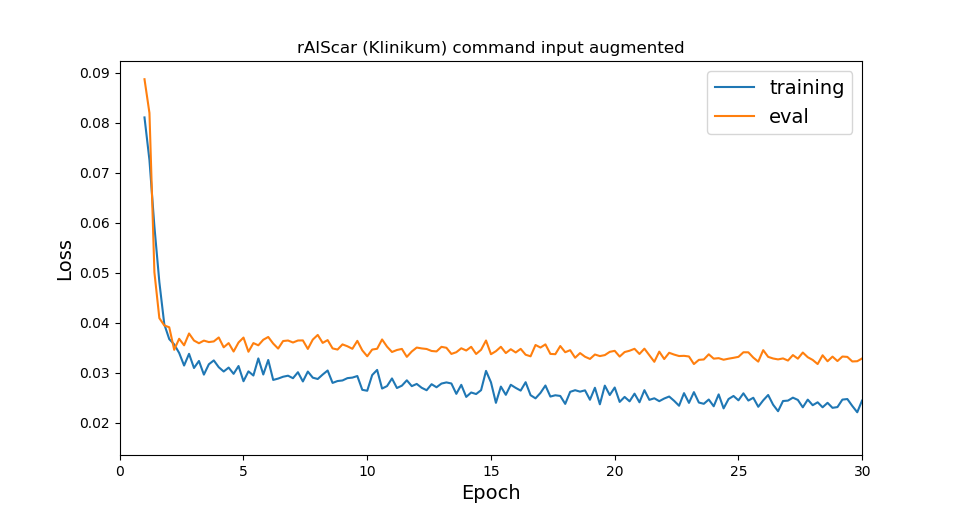
\includegraphics[width=0.95\textwidth]{figures/klinikum_command_input_aug_lossplot}
  \caption{Klinikum rAIScar command input lossplot}
  \label{fig:klinikum_augmented_command_loss}
\end{figure}
\begin{figure}[!htbp]
  \centering
  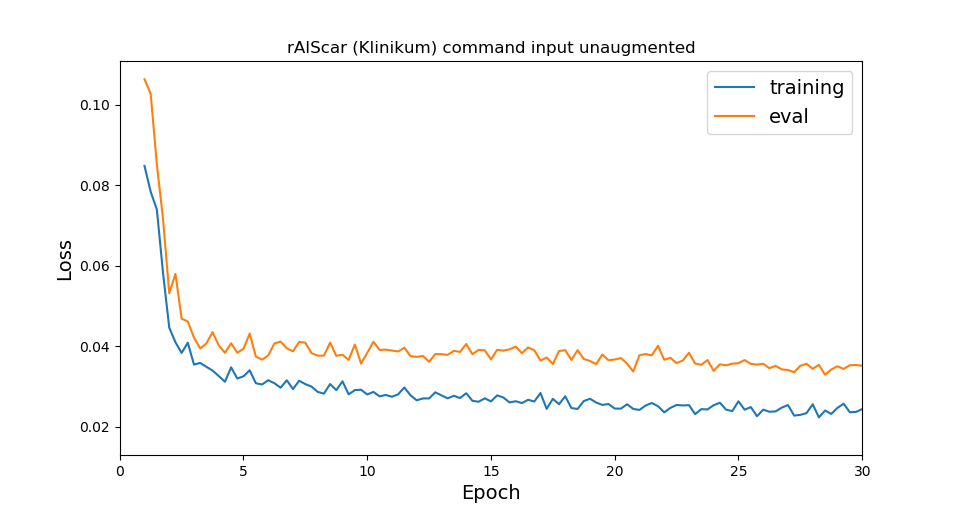
\includegraphics[width=0.95\textwidth]{figures/klinikum_command_input_nonaug_lossplot}
  \caption{Klinikum rAIScar command input, unaugmented lossplot}
  \label{fig:klinikum_unaugmented_command_loss}
\end{figure}
\begin{figure}[H]
\centering
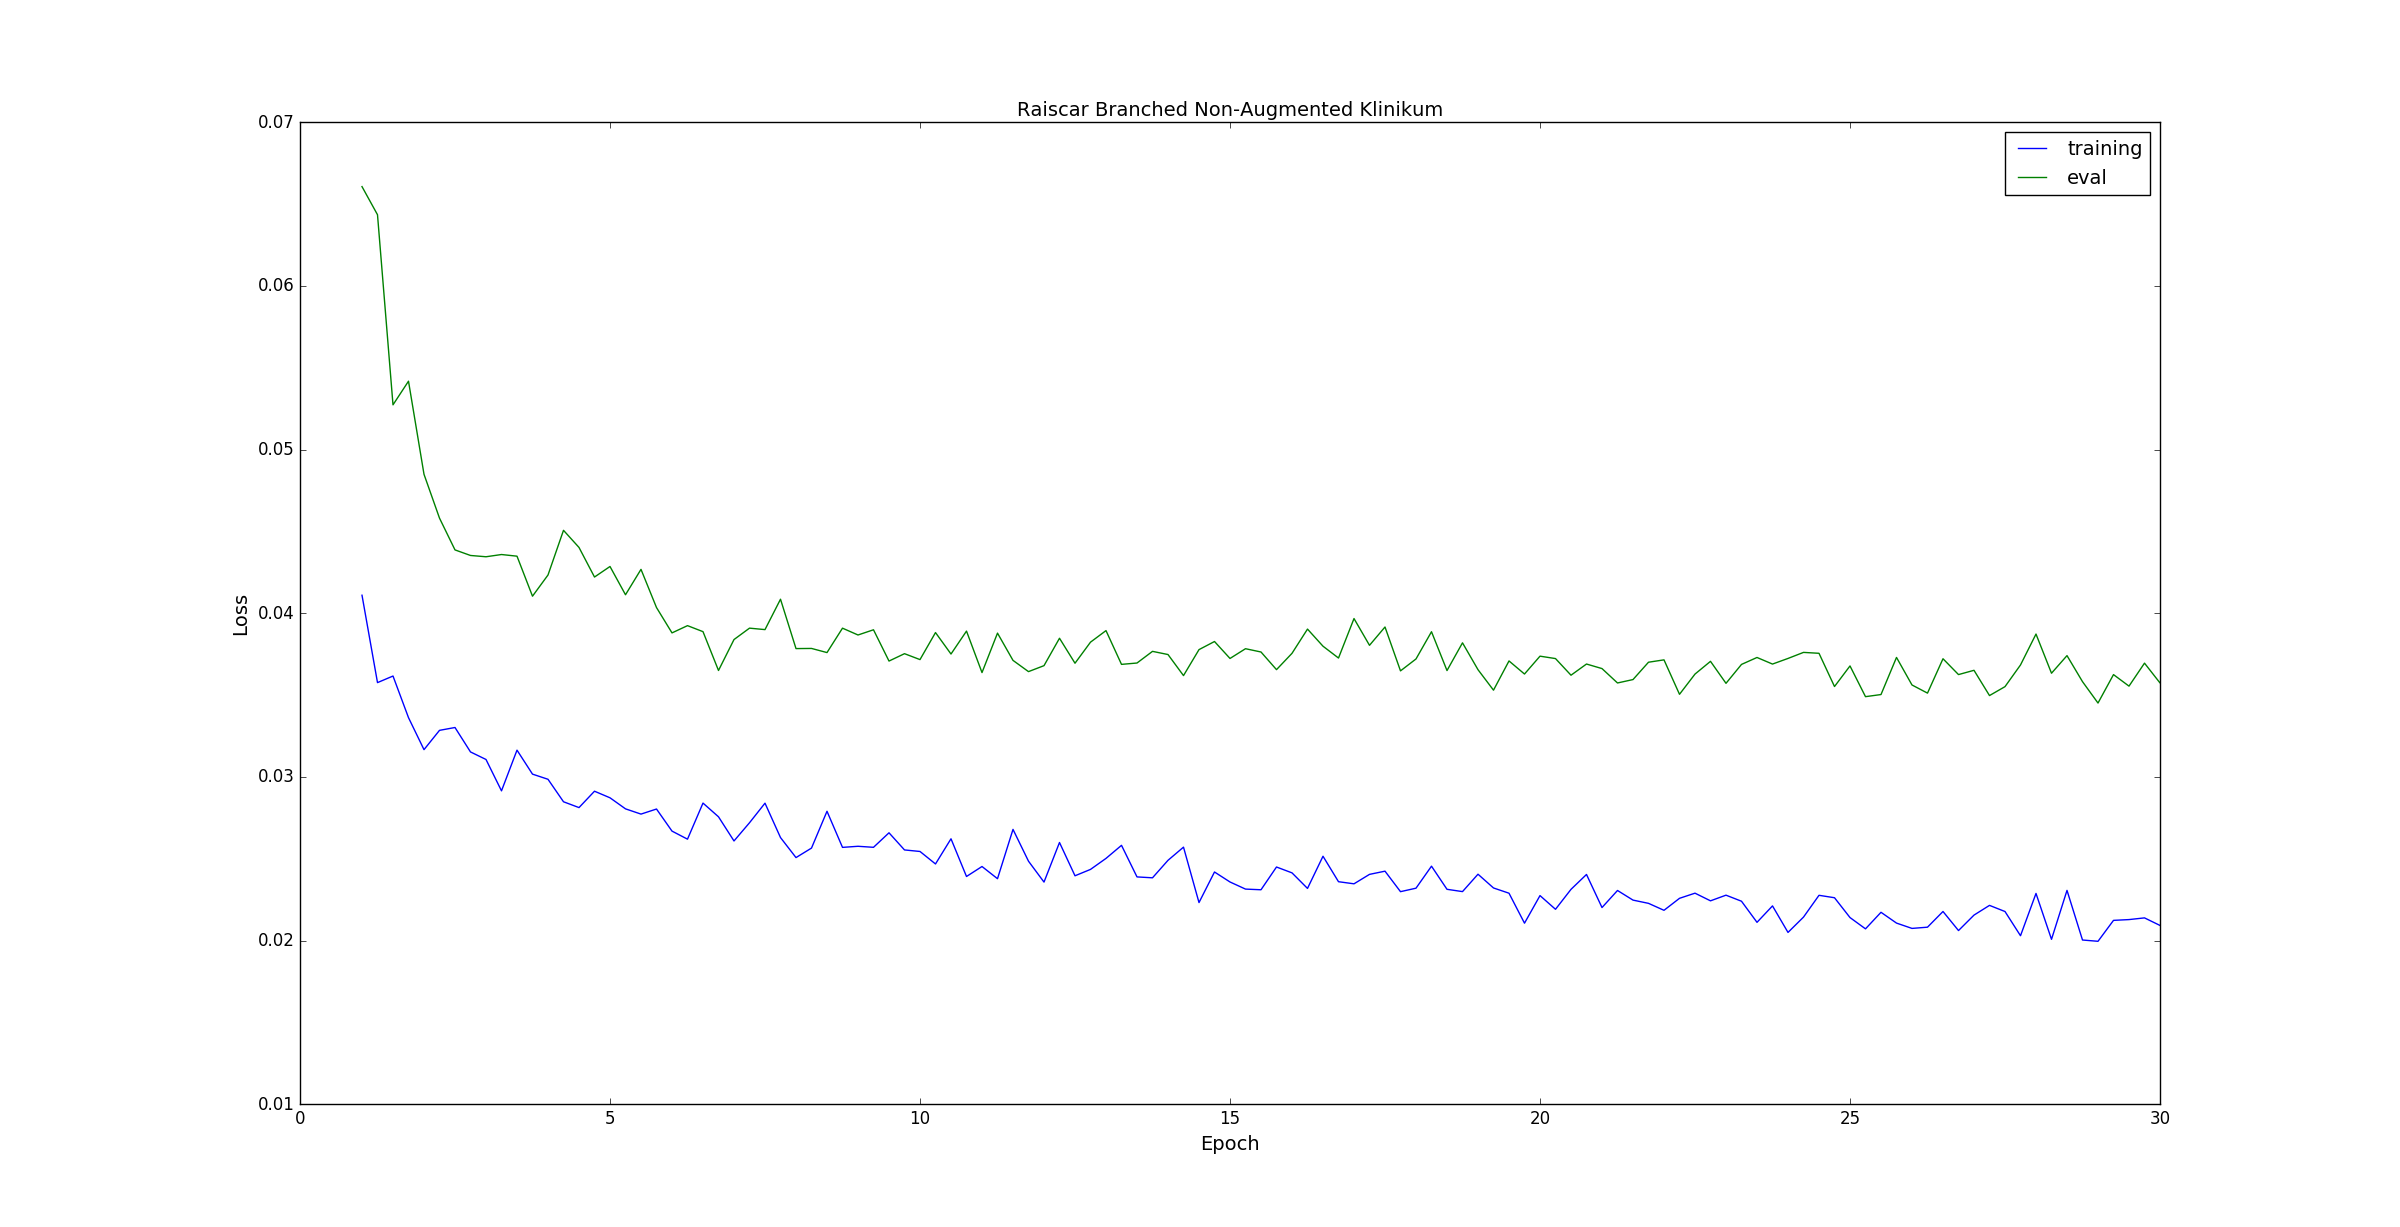
\includegraphics[width=0.95\textwidth]{figures/raiscar_branched_non_aug_klinikum_lossplot}
\caption{Klinikum rAIScar branched, unaugmented lossplot}
\label{fig:klinikum_unaugmented_branched_loss}
\end{figure}
\begin{figure}[H]
	\centering
	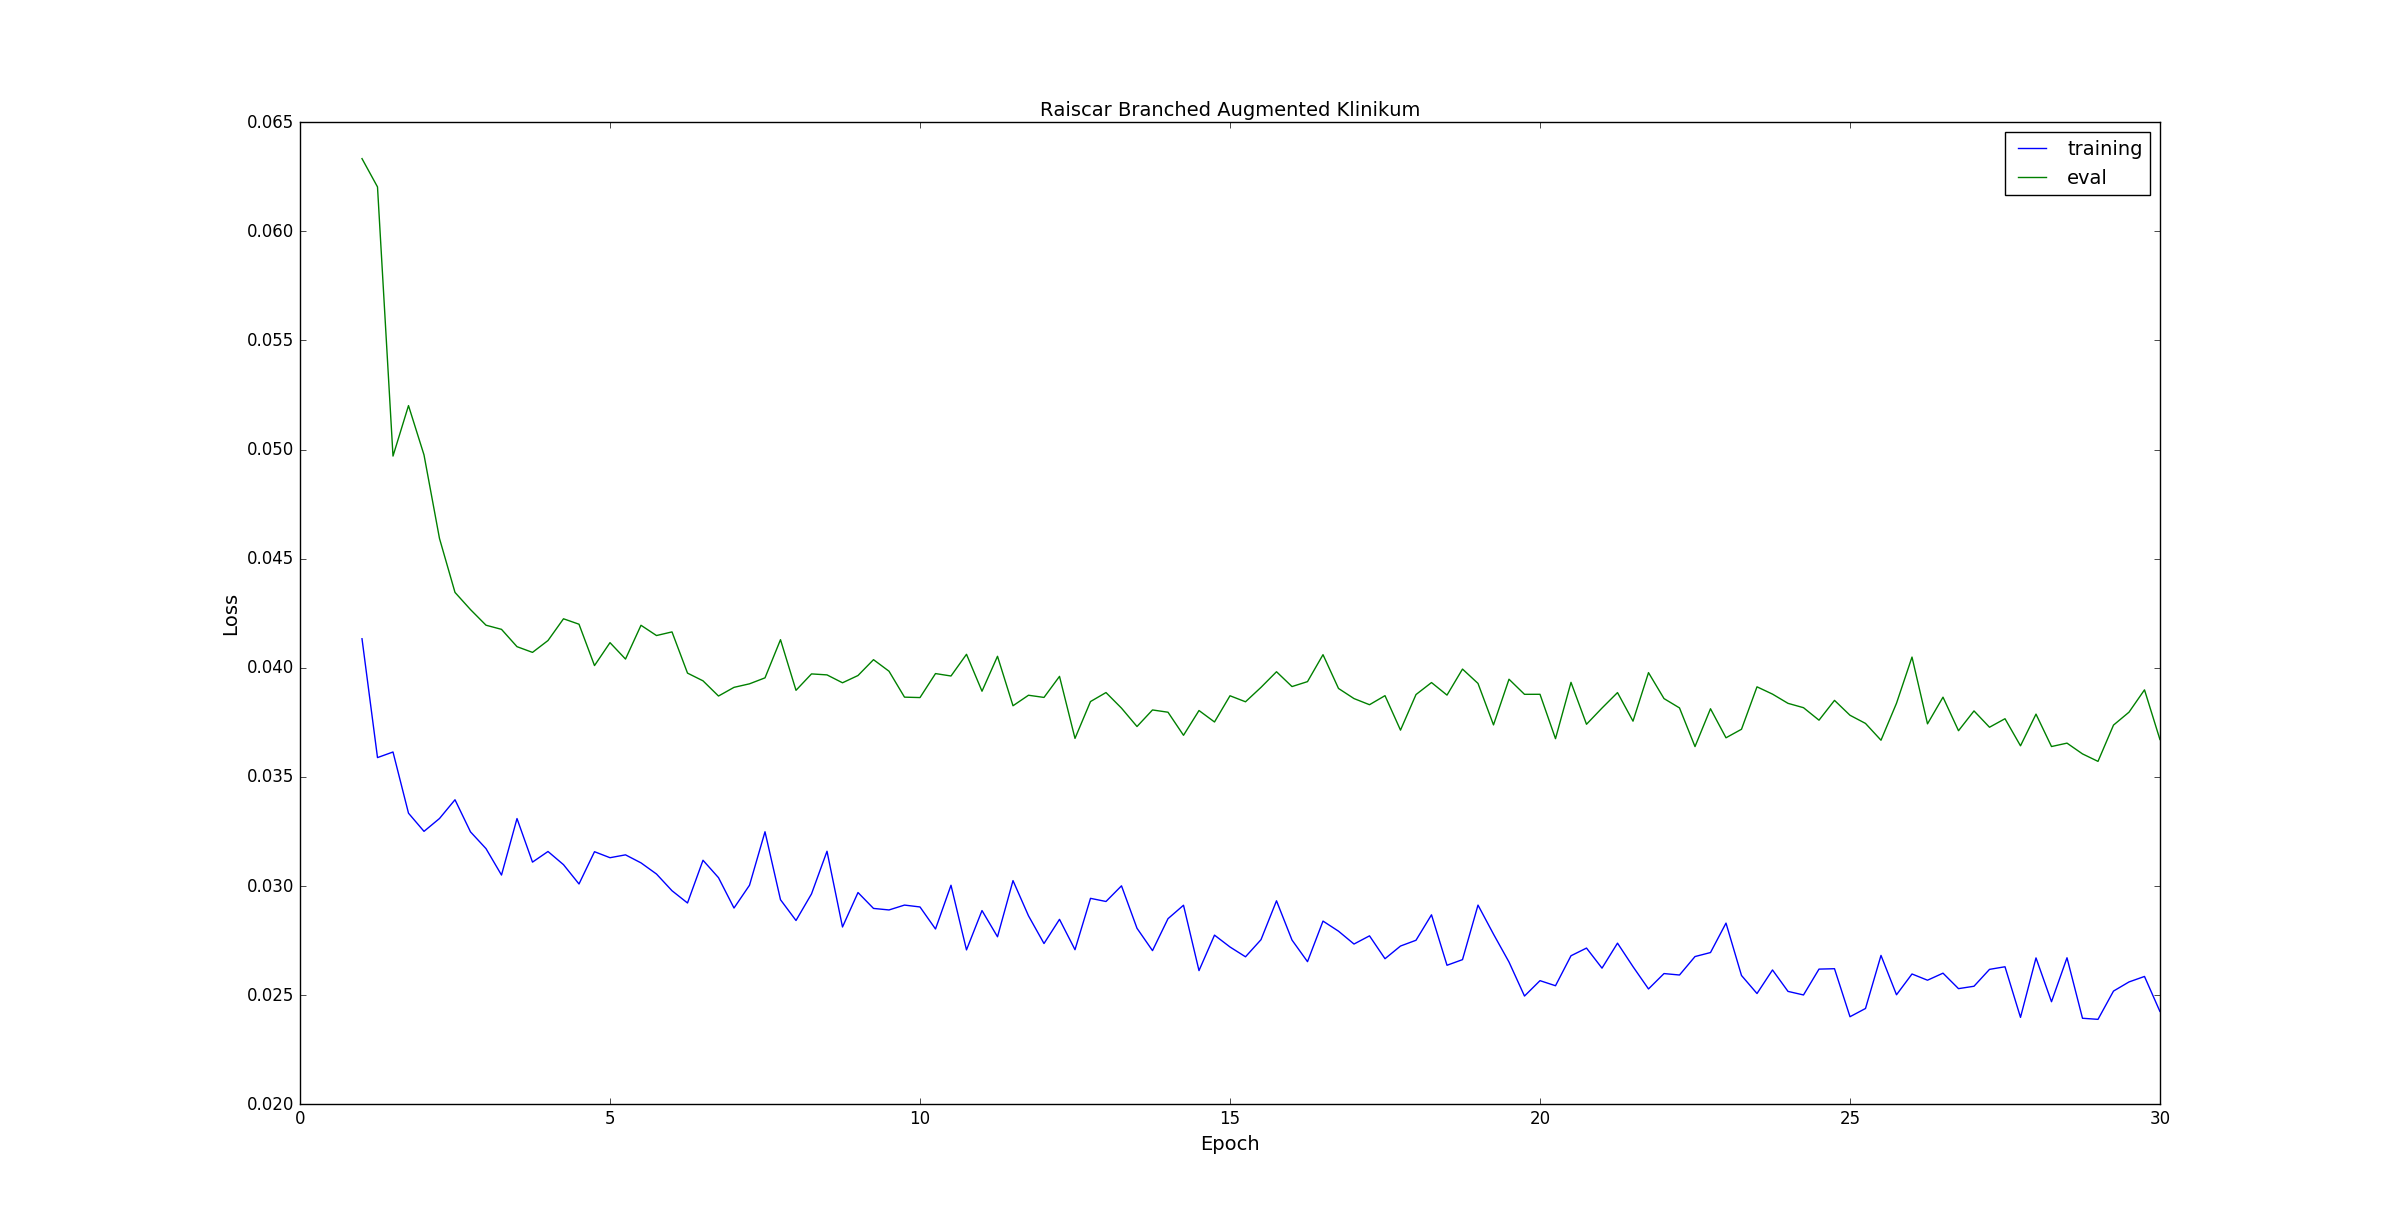
\includegraphics[width=0.95\textwidth]{figures/raiscar_branched_aug_klinikum_lossplot}
	\caption{Klinikum rAIScar branched, augmented lossplot}
	\label{fig:klinikum_augmented_branched_loss}
\end{figure}

\subsection{Interpretation}
For the command input net, the results from the lossplot and testing diverge.
While the augmented evaluation loss is marginally better in the augmentated run,
the testing error is way worse, which can also be seen in the testing video.

This discrepancy doesn't appear in the branched network, where augmentation
doesn't seem to have any bigger influence on the evaluation loss and testing
error.

\section{Improvements}
The Klinikum dataset had several issues. Firstly, the roads have a relatively
big elevation variance and have quite diverging optics (ocre bricks vs.
pavement). Also, since we weren't as experienced driving the rAIScar, the
steering motions where quite jerky, which makes it more difficult for the net to
be trained correctly.

We already took another training set on the old Freiburg cemetery, which has a
more interesting layout, steady elevation, narrower roads and more experienced
drivers, which we are currently in the process of training.


\begin{thebibliography}{9}
\bibitem{imitation}
Codevilla, Felipe and Müller, Matthias and López, Antonio and Koltun, Vladlen
and Dosovitskiy, Alexey.
\textit{End-to-end Driving via Conditional Imitation Learning.}
ICRA 2018
\end{thebibliography}
\end{document}